% Shared preamble for the CIG-AMF formal-research papers.
% IEEEtran conference class; compiles on Overleaf without modification.
\documentclass[conference]{IEEEtran}
\IEEEoverridecommandlockouts

\usepackage{cite}
\usepackage{amsmath,amssymb,amsfonts}
\usepackage{amsthm}
\usepackage{algorithm}
\usepackage{algorithmic}
\usepackage{graphicx}
\usepackage{textcomp}
\usepackage{xcolor}
\usepackage{booktabs}
\usepackage{url}
\usepackage[hidelinks]{hyperref}

\def\BibTeX{{\rm B\kern-.05em{\sc i\kern-.025em b}\kern-.08em T\kern-.1667em\lower.7ex\hbox{E}\kern-.125emX}}

\newtheorem{theorem}{Theorem}
\newtheorem{lemma}[theorem]{Lemma}
\newtheorem{proposition}[theorem]{Proposition}
\newtheorem{corollary}[theorem]{Corollary}
\theoremstyle{definition}
\newtheorem{definition}[theorem]{Definition}
\newtheorem{remark}[theorem]{Remark}
\newtheorem{example}[theorem]{Example}

% A machine-checked statement carries its Lean declaration name.
\newcommand{\lean}[1]{\textsf{\footnotesize #1}}
\newcommand{\leanbox}[1]{%
  \par\vspace{2pt}\noindent
  {\footnotesize\textsf{Lean: #1}}\par\vspace{2pt}}

% Evidence classes, used consistently and never interchangeably.
\newcommand{\PROVED}{\textsc{proved}}
\newcommand{\CERT}{\textsc{certificate}}
\newcommand{\NUM}{\textsc{numerical}}
\graphicspath{{../_figures/}}


\begin{document}

\title{House Monotonicity and Quota Cannot Both Hold:\\
Closing the Probabilistic Inputs of an\\
Adaptive Stopping Analysis}

\author{\IEEEauthorblockN{Vu Phan An Nguyen}
\IEEEauthorblockA{\textit{Rider University} \\
Lawrenceville, NJ, USA}}

\maketitle

\begin{abstract}
An adaptive scheme allocates samples across arms, stops when a certificate is available, and
must be analysed on three fronts: the probability that its confidence event holds, the
expected time at which it stops, and whether its realised counts follow the intended
proportions. Three claims in that analysis were carried without proof, and they were carried
in three different ways. The per-arm concentration inequality appeared as a hypothesis of the
enclosing lemma, so a reader could see it but nothing established that anything satisfies it.
The step from a tail bound to a bound on the \emph{expected} stopping time was cited in a
comment as standard, which is weaker, since a comment does not appear in the statement. And
the tracking bound was taken for granted in prose describing what the sampling rule does,
which is the worst position of the three: an assumption nobody wrote down is one nobody
checked. This paper closes all three, and the third has a negative answer that is itself the
result. We prove the layer-cake identity for an $\mathbb{N}$-valued stopping time, so a
geometric tail bounds the expected stopping time rather than merely the tail sum. We discharge
the concentration input from a sub-Gaussian hypothesis at an explicit threshold. We prove by
construction that for every target and every horizon there \emph{exists} an integer allocation
spending exactly the horizon with per-arm deficit at most one. And we show that the natural
online rule---serve the arm of largest deficit, which is house-monotone by construction---does
\emph{not} achieve it, on an exact five-arm witness reaching deficit $\tfrac{26}{23}$ at
horizon eleven. An exhaustive search over $5{,}070$ rational targets finds $1{,}147$ that
violate the bound, the worst reaching $\tfrac32$ and the earliest at $t=3$.
\end{abstract}

\begin{IEEEkeywords}
adaptive sampling, stopping times, concentration inequalities, apportionment,
house monotonicity, quota, formal verification
\end{IEEEkeywords}

\section{Introduction}

An adaptive sampling scheme decides at each round which arm to sample, stops when the data
support a certificate, and its guarantee has two parts: the recommendation is correct with
probability at least $1-\delta$, and the expected stopping time is bounded.

The two parts are proved differently, and it is easy to let the first do the second's work.
Correctness follows from a union bound over confidence intervals---the good event---and is
where a concentration input enters. The stopping-time bound cannot follow from the good event,
because that event says nothing about its complement, and on the complement the scheme may
draw forever. It follows instead from a tail bound on the stopping time itself, and converting
that tail into an expectation is the layer-cake step. Citing that step is reasonable in prose
and inadequate in a development that claims its results are checked.

Between the two sits the sampling rule. The tail bound is obtained by showing that after
enough rounds the statistic must cross, and ``enough'' is computed from how many samples each
arm has by then---which is where the intended proportions enter, and where the tracking
question lives. Writing $D_{i}(t)=t\,w_{i}-N_{i}(t)$ for the deficit of arm $i$ against target
$w$, an analysis would like to assume $|D_{i}(t)|\le1$ at every horizon.

This paper proves such an allocation always \emph{exists} and that the natural online rule does
not \emph{achieve} it. The two together say the bound is true as an existence statement and
false as a property of the rule an algorithm would use, which is exactly the distinction an
analysis must respect. The obstruction is the apportionment paradox in algorithmic form: house
monotonicity---counts only increase as the horizon grows---and quota cannot both hold.

The paper makes five contributions. First, it proves the layer-cake identity, so a geometric
tail bounds the expected stopping time. Second, it discharges the concentration input from a
sub-Gaussian hypothesis at an explicit threshold. Third, it proves the per-horizon existence
by construction rather than by an existence argument. Fourth, it refutes the online bound with
an exact witness whose eleven steps are each a genuine largest-deficit choice. Fifth, it
states the transfer an analysis actually consumes with the constant left free, so that
whatever bound a specific rule can prove may be substituted.

The scope is bounded. The refutation concerns \emph{this} rule and does not prove that no
online monotone rule achieves any constant bound; the search establishing how common the
failure is covers a finite family; the concentration result assumes a known sub-Gaussian
parameter; and the geometric tail itself remains an input supplied by the algorithm's own
analysis.

\section{Background}

\subsection{Fixed-Confidence Sampling}

Garivier and Kaufmann establish the framework in which this analysis sits: a stopping rule
based on a generalised likelihood-ratio statistic, a sampling rule that tracks the
optimal-allocation weights, and a sample-complexity bound matching a lower bound
asymptotically \cite{garivier2016}. Kaufmann, Capp\'e and Garivier give the complexity of
best-arm identification in the general bandit model \cite{kaufmann2016}. The tracking device
in that framework is the direct source of the question
Sections~\ref{sec:exists}--\ref{sec:fails} answer, and the concentration inputs are the ones
Section~\ref{sec:subgauss} discharges.

Nothing here improves their bounds. What is contributed is that two of the analysis's inputs
become theorems in this development, and that the tracking assumption is shown to be
unavailable in the form an analysis would most like to use.

\subsection{Apportionment}

Balinski and Young prove the impossibility at the heart of the negative result: no
apportionment method satisfies both house monotonicity and quota, so divisor methods are
house-monotone and violate quota while quota methods violate house monotonicity
\cite{balinski1982}. That result is stated in the language of seats and states, for
apportionment methods in general.

Theorem~\ref{thm:quotafails} is not a restatement of it, and the difference is what makes it
usable. The general impossibility says \emph{some} violation exists for any house-monotone
method. The witness says \emph{this} rule violates quota at $t=11$ on
$\frac{1}{23}(17,1,1,3,1)$ by $\frac{26}{23}$. An analysis that assumes a unit deficit bound
needs the second, not the first: it needs a horizon, a target and a magnitude. The connection
to \cite{balinski1982} is acknowledged and is why the failure is unsurprising in hindsight.

\subsection{Concentration}

The sub-Gaussian Chernoff bound of Section~\ref{sec:subgauss} is standard
\cite{boucheron2013}, as is the measure-theoretic apparatus behind the layer-cake identity
\cite{durrett2019}. Both are proved here because the peeling argument needs the first at a
specific threshold with a specific budget, and because the point of the exercise is to have no
assumed inequalities left.

\subsection{The Gap}

The literature therefore leaves a specific opening. The fixed-confidence framework supplies
the analysis but carries concentration and layer-cake as inputs; apportionment supplies a
general impossibility but no instance an analysis can use; concentration theory supplies the
inequality but not its instantiation at the peeling budget. No existing treatment
simultaneously: (i) proves the layer-cake transfer for the $\mathbb{N}$-valued stopping time
the analysis needs; (ii) discharges the per-arm concentration input at the peeling budget;
(iii) separates per-horizon existence from online achievability by proving the first and
refuting the second; and (iv) quantifies how common and how early the online failure is.

\section{Research Aims, Questions, and Hypotheses}

\subsection{Research Aim}

The aim of this work is to remove the unproved inputs from an adaptive stopping analysis and
to determine whether the tracking bound that analysis relies on is achievable by an online
rule.

\subsection{Research Questions}

\begin{itemize}
\item \textbf{RQ1.} Does a geometric tail on the stopping time bound its expectation, as a
theorem rather than a citation?
\item \textbf{RQ2.} Can the per-arm, per-count concentration inequality be supplied rather
than assumed, at the budget the peeling argument allocates?
\item \textbf{RQ3.} Does an integer allocation with per-arm deficit at most one exist at every
horizon?
\item \textbf{RQ4.} Does the natural online monotone rule achieve that bound?
\end{itemize}

\subsection{Hypotheses}

\begin{itemize}
\item \textbf{H1.} Writing the stopping time as a sum of indicators and exchanging with the
integral gives the layer-cake identity, from which a geometric tail yields $C/(1-\rho)$.
\item \textbf{H2.} A sub-Gaussian deviation meets any budget $\beta$ at threshold
$\sqrt{2c\log(1/\beta)}$, which is what the peeling budget requires.
\item \textbf{H3.} Taking floors and distributing the shortfall one unit per arm gives an
allocation with deficit at most one, at every horizon.
\item \textbf{H4.} The online rule does not achieve it, and the failure is neither rare nor
asymptotic.
\end{itemize}

\section{Methodology}
\label{sec:setting}

\subsection{Framework Overview}

An allocation rule is \emph{house-monotone} when $N_{i}(t)$ is non-decreasing in $t$ for every
$i$---no arm's count ever falls as the horizon grows. It satisfies \emph{quota} at constant
$c$ when $|D_{i}(t)|\le c$ for every $i$ and $t$. Any rule serving one arm per round is
house-monotone by construction, since counts only increase; that is why the natural online
rule sits on one side of the impossibility automatically.

\subsection{Simplifying Assumptions}

\begin{enumerate}
\item[1)] \textbf{Known sub-Gaussian parameter.} Theorem~\ref{thm:subgauss} assumes the
deviation is sub-Gaussian with a \emph{known} parameter $c$. Gaussian noise satisfies this, so
the hypothesis is met in the intended setting; with an estimated variance it is not automatic,
and nothing here covers that case.

\item[2)] \textbf{Geometric tail as an input.} Corollary~\ref{cor:expstop} converts a
geometric tail into an expectation bound. Establishing the tail is the algorithm's own
analysis and is not done here.

\item[3)] \textbf{One sample per round.} The rule serves exactly one arm per round, which is
what makes it house-monotone and what makes the granularity argument of
Section~\ref{sec:reading} apply.

\item[4)] \textbf{Targets on the simplex.} $w$ is non-negative and sums to one, which is what
makes the deficits sum to zero in Lemma~\ref{lem:sumzero}.
\end{enumerate}

\subsection{The Layer-Cake Identity}
\label{sec:layercake}

\begin{theorem}[Layer cake for an $\mathbb{N}$-valued stopping time]
\label{thm:layercake}
For an $\mathbb{N}$-valued measurable $\tau$,
\begin{equation}
\int \tau \,d\mu\;=\;\sum_{n\geq 0}\mu\{\tau>n\}.
\label{eq:layercake}
\end{equation}
\end{theorem}

\begin{proof}
At each point write $\tau=\sum_{n\ge0}\mathbf{1}\{n<\tau\}$, a sum with exactly $\tau$
non-zero terms which telescopes to the value itself. Exchange the sum with the integral, which
is legitimate for non-negative measurable terms by monotone convergence.
\end{proof}

\leanbox{\lean{lintegral\_nat\_eq\_tsum\_meas\_gt} in
\lean{LeanAdaptiveExpectedStoppingV1}}

The $\mathbb{N}$-valued case is stated separately rather than derived from the general
layer-cake formula for non-negative functions, because the integer case yields a countable sum
rather than an integral over levels, and the countable form is what the next statement needs
in order to sum a geometric series.

\begin{corollary}[Geometric tail bounds the expectation]
\label{cor:expstop}
If $\mu\{\tau>n\}\le C\rho^{n}$ with $0\le\rho<1$, then
$\mathbb{E}[\tau]\le C/(1-\rho)$.
\end{corollary}

\leanbox{\lean{expected\_stopping\_le} in \lean{LeanAdaptiveExpectedStoppingV1}}

The hypothesis $\rho<1$ is explicit because an earlier version omitted it; the statement is
then false, and the omission is invisible in prose because ``geometric tail'' carries the
condition informally.

\subsection{The Concentration Input}
\label{sec:subgauss}

\begin{theorem}[Sub-Gaussian threshold]
\label{thm:subgauss}
If $X$ is sub-Gaussian with parameter $c\ge0$, then for any budget $\beta\in(0,1)$,
\begin{equation}
\mu\Bigl\{\sqrt{2c\log(1/\beta)}\leq X\Bigr\}\;\leq\;\beta .
\label{eq:subgauss}
\end{equation}
\end{theorem}

\begin{proof}
The sub-Gaussian Chernoff bound gives $\mu\{X\ge u\}\le\exp(-u^{2}/2c)$; evaluating at
$u=\sqrt{2c\log(1/\beta)}$ makes the exponent $-\log(1/\beta)$.
\end{proof}

\leanbox{\lean{subgaussian\_threshold} in \lean{LeanAdaptiveExpectedStoppingV1}}

The threshold is stated in terms of an arbitrary budget $\beta$ rather than a fixed
$\delta$ because that is the form the peeling argument consumes: it allocates
$\delta/(K\,n(n+1))$ to arm $i$ at count $n$---the factor chosen so that
$\sum_{n\ge1}1/(n(n+1))=1$---and \eqref{eq:subgauss} converts that budget into an interval
half-width. Without it the peeling argument has a budget and no way to spend it.

\subsection{Deficits, and Why a Greedy Rule Never Idles}
\label{sec:deficits}

\begin{lemma}[Deficits sum to zero]
\label{lem:sumzero}
$D_{i}(t)=t\,w_{i}-N_{i}(t)$ satisfies $\sum_{i} D_{i}(t)=0$.
\end{lemma}

\begin{proof}
$\sum_{i}D_{i}(t)=t\sum_{i}w_{i}-\sum_{i}N_{i}(t)=t-t=0$.
\end{proof}

\leanbox{\lean{deficit\_sum\_zero} in \lean{LeanAdaptiveTrackingV1}}

\begin{corollary}[Some arm is always behind]
\label{cor:deficient}
$\max_{i}D_{i}(t)\ge0$ for every $t$.
\end{corollary}

\begin{proof}
A finite family of reals summing to zero cannot be everywhere negative.
\end{proof}

\leanbox{\lean{exists\_deficient} in \lean{LeanAdaptiveTrackingV1}}

Corollary~\ref{cor:deficient} is elementary and is stated because it is what makes the greedy
rule well defined: there is always an arm with non-negative deficit to serve, so the rule's
argmax is meaningful at every horizon. The alternative is an implicit assumption to that
effect.

\subsection{A Tracking Allocation Exists}
\label{sec:exists}

\begin{theorem}[Existence at every horizon]
\label{thm:exists}
\begin{equation}
\forall\,w,\;\forall\,t:\;\;
\exists\,N:\;\;\sum_{i} N_{i}=t
\;\;\text{and}\;\;\bigl|N_{i}-t\,w_{i}\bigr|\leq 1 .
\label{eq:exists}
\end{equation}
\end{theorem}

\begin{proof}[Construction]
Take $N_{i}^{0}=\lfloor t\,w_{i}\rfloor$. Then $\sum_{i}N_{i}^{0}\le t$, and the shortfall is
strictly less than $K$ because each floor loses less than one. Distribute the shortfall one
unit per arm over a subset of that size; every count then lies between
$\lfloor t\,w_{i}\rfloor$ and $\lfloor t\,w_{i}\rfloor+1$.
\end{proof}

\leanbox{\lean{tracking\_bound}, \lean{tracking\_exists} in \lean{LeanAdaptiveTrackingV1}}

The construction uses floors and a correction set and nothing else, so the allocation can be
written down for any $(w,t)$. But it is per-horizon: for each $t$ separately it gives an
allocation meeting the bound. It does \emph{not} give a single rule whose counts are monotone
in $t$ and meet the bound at every $t$ simultaneously, and that stronger statement is what an
algorithm needs.

\subsection{The Online Rule Fails Quota}
\label{sec:fails}

\begin{theorem}[Largest-deficit-first violates quota]
\label{thm:quotafails}
On five arms with targets $w=\frac{1}{23}(17,1,1,3,1)$, the rule serving the arm of largest
deficit reaches counts $(7,1,1,1,1)$ after eleven steps, at which point
\begin{equation}
D_{0}(11)\;=\;11\cdot\frac{17}{23}-7\;=\;\frac{26}{23}\;>\;1 .
\label{eq:quotafail}
\end{equation}
Continuing to horizon fourteen the deficit reaches $\frac{31}{23}$.
\end{theorem}

\leanbox{\lean{weights\_sum\_one}, \lean{counts\_sum}, \lean{deficit\_exceeds\_one},
\lean{online\_quota\_fails} in \lean{LeanAdaptiveOnlineQuotaFailsV1}}

\begin{table*}[t]
\caption{Every step of the largest-deficit rule on targets
$w=\frac{1}{23}(17,1,1,3,1)$, in exact rationals. Column $D_{i}(t)=t\,w_{i}-N_{i}(t)$ is the
deficit before the step; the served arm is the one attaining the maximum, checked against
every other arm at every step, so the counts are what the \emph{rule} produces and not a
tie-breaking accident. The deficits sum to zero in every row
(Lemma~\ref{lem:sumzero}). At $t=11$ the first arm's deficit is
$\frac{26}{23}\approx1.130$, exceeding the per-horizon bound of one that
Theorem~\ref{thm:exists} guarantees is achievable offline; by $t=14$ it reaches
$\frac{31}{23}\approx1.348$.}
\label{tab:trace}
\centering
\footnotesize
\setlength{\tabcolsep}{5pt}
\begin{tabular}{@{}rlrrrrrcl@{}}
\toprule
$t$ & $N(t)$ & $D_{0}$ & $D_{1}$ & $D_{2}$ & $D_{3}$ & $D_{4}$ & serve & \\
\midrule
0 & $(0,0,0,0,0)$ & $0$ & $0$ & $0$ & $0$ & $0$ & 0 &  \\
1 & $(1,0,0,0,0)$ & $-\frac{6}{23}$ & $\frac{1}{23}$ & $\frac{1}{23}$ & $\frac{3}{23}$ & $\frac{1}{23}$ & 3 &  \\
2 & $(1,0,0,1,0)$ & $\frac{11}{23}$ & $\frac{2}{23}$ & $\frac{2}{23}$ & $-\frac{17}{23}$ & $\frac{2}{23}$ & 0 &  \\
3 & $(2,0,0,1,0)$ & $\frac{5}{23}$ & $\frac{3}{23}$ & $\frac{3}{23}$ & $-\frac{14}{23}$ & $\frac{3}{23}$ & 0 &  \\
4 & $(3,0,0,1,0)$ & $-\frac{1}{23}$ & $\frac{4}{23}$ & $\frac{4}{23}$ & $-\frac{11}{23}$ & $\frac{4}{23}$ & 1 &  \\
5 & $(3,1,0,1,0)$ & $\frac{16}{23}$ & $-\frac{18}{23}$ & $\frac{5}{23}$ & $-\frac{8}{23}$ & $\frac{5}{23}$ & 0 &  \\
6 & $(4,1,0,1,0)$ & $\frac{10}{23}$ & $-\frac{17}{23}$ & $\frac{6}{23}$ & $-\frac{5}{23}$ & $\frac{6}{23}$ & 0 &  \\
7 & $(5,1,0,1,0)$ & $\frac{4}{23}$ & $-\frac{16}{23}$ & $\frac{7}{23}$ & $-\frac{2}{23}$ & $\frac{7}{23}$ & 2 &  \\
8 & $(5,1,1,1,0)$ & $\frac{21}{23}$ & $-\frac{15}{23}$ & $-\frac{15}{23}$ & $\frac{1}{23}$ & $\frac{8}{23}$ & 0 &  \\
9 & $(6,1,1,1,0)$ & $\frac{15}{23}$ & $-\frac{14}{23}$ & $-\frac{14}{23}$ & $\frac{4}{23}$ & $\frac{9}{23}$ & 0 &  \\
10 & $(7,1,1,1,0)$ & $\frac{9}{23}$ & $-\frac{13}{23}$ & $-\frac{13}{23}$ & $\frac{7}{23}$ & $\frac{10}{23}$ & 4 &  \\
11 & $(7,1,1,1,1)$ & $\frac{26}{23}$ & $-\frac{12}{23}$ & $-\frac{12}{23}$ & $\frac{10}{23}$ & $-\frac{12}{23}$ & 0 & $>1$ \\
12 & $(8,1,1,1,1)$ & $\frac{20}{23}$ & $-\frac{11}{23}$ & $-\frac{11}{23}$ & $\frac{13}{23}$ & $-\frac{11}{23}$ & 0 &  \\
13 & $(9,1,1,1,1)$ & $\frac{14}{23}$ & $-\frac{10}{23}$ & $-\frac{10}{23}$ & $\frac{16}{23}$ & $-\frac{10}{23}$ & 3 &  \\
14 & $(9,1,1,2,1)$ & $\frac{31}{23}$ & $-\frac{9}{23}$ & $-\frac{9}{23}$ & $-\frac{4}{23}$ & $-\frac{9}{23}$ & 0 & $>1$ \\
\bottomrule
\end{tabular}
\end{table*}


A counterexample to a rule's behaviour is only as good as the claim that the trace is what the
rule produces, so Table~\ref{tab:trace} records the deficit of every arm at every step and the
served arm is compared against each alternative rather than asserted to be the argmax. At every
step in the table the maximum is attained uniquely, so any implementation of
largest-deficit-first produces these counts whatever it does about ties.

\subsection{What Is Machine-Checked Here, and What Is Not}
\label{sec:gap}

This paper's subject is inputs carried without proof, so the evidence behind
Theorem~\ref{thm:quotafails} is separated rather than summarised.

\emph{Machine-checked.} That $w$ lies on the simplex; that the count vector spends exactly
eleven pulls; and that $11\,w_{0}-N_{0}>1$ in exact rational arithmetic. Together these prove:
there is a target on the simplex and an allocation of eleven pulls whose first-arm deficit
exceeds one.

\emph{Not machine-checked.} That $N=(7,1,1,1,1)$ is the allocation the largest-deficit rule
actually reaches. The eleven step comparisons sit in the proof body of a lemma whose conclusion
is \lean{True}, written as hardcoded rationals; each is kernel-checked as an arithmetic fact,
but nothing about them is exported and no statement connects those literals to $w$ and $N$.
The rule-to-counts link---the part that makes this a statement about the \emph{rule} rather
than about some allocation---is carried by a comment in the module, not by a proof.

\emph{How the link is established instead.} We recomputed the trajectory independently in
exact rational arithmetic, simulating largest-deficit-first on $w$ from $t=0$ and comparing
the served arm against all four alternatives at every step. It reproduces
Table~\ref{tab:trace} exactly, including the serve order $[0,3,0,0,1,0,0,2,0,0,4]$, the counts
$(7,1,1,1,1)$ and $D_{0}(11)=\frac{26}{23}$. That computation is a \NUM{} result: exact,
reproducible, and not machine-checked.

Theorem~\ref{thm:quotafails} should therefore be read as one \PROVED{} half and one \NUM{}
half. Closing the gap means formalising the greedy rule as a Lean function and proving
$\mathrm{greedyCount}(w,11)=N$, which is not done.

\subsection{What the Analysis Actually Consumes}
\label{sec:consumes}

\begin{theorem}[Deficit bound transfers to frequencies]
\label{thm:freq}
\begin{equation}
\bigl|N_{i}-t\,w_{i}\bigr|\leq c
\qquad\Longrightarrow\qquad
\left|\frac{N_{i}}{t}-w_{i}\right|\;\leq\;\frac{c}{t} .
\label{eq:freq}
\end{equation}
\end{theorem}

\leanbox{\lean{frequency\_converges}, \lean{pull\_count\_lower} in
\lean{LeanAdaptiveTrackingV1}}

Theorem~\ref{thm:freq} is stated with $c$ free for a reason. Whatever bound a specific rule can
prove---not the $c=1$ that Section~\ref{sec:fails} refutes---converts into a statement about
empirical proportions at rate $c/t$, and a companion bound converts it into a lower bound on
pull counts between any two times, which is what a peeling argument needs.

\section{Formal Verification}
\label{sec:verification}

\subsection{Acceptance Contract}

A module counts as accepted only when all six of the following hold: the compiler exits zero
with no errors; the source hash is unchanged \emph{across} the compile, so the file checked is
the file on disk; the compiled artifact is newer than its source; at least one
\texttt{\#print axioms} directive is present; the axiom set of every audited declaration lies
within $\{\textsf{propext},\textsf{Classical.choice},\textsf{Quot.sound}\}$; and no
\texttt{sorry} appears anywhere in the file.

The contract is stated in full because each clause excludes a specific way of appearing
verified without being so. The hash check across the compile excludes editing a file after
checking it; the artifact-newer check excludes a stale \texttt{.olean}; and the axiom audit is
a \emph{whitelist} rather than a blacklist, so an axiom introduced by a decision procedure
outside the kernel is rejected by name mismatch rather than needing to be anticipated.

\subsection{Evidence per Step}

\begin{table}[htbp]
\caption{Evidence per step. All cited declarations are axiom-audited.}
\label{tab:inventory}
\centering\footnotesize\setlength{\tabcolsep}{3pt}
\begin{tabular}{@{}llr@{}}
\toprule
Step & Module & Aud. \\
\midrule
Layer cake, Thm~\ref{thm:layercake}   & \lean{LeanAdaptiveExpectedStoppingV1}  & 3 \\
Concentration, Thm~\ref{thm:subgauss} & \lean{LeanAdaptiveExpectedStoppingV1}  & 3 \\
Deficits, Lem~\ref{lem:sumzero}       & \lean{LeanAdaptiveTrackingV1}          & 6 \\
Existence, Thm~\ref{thm:exists}       & \lean{LeanAdaptiveTrackingV1}          & 6 \\
Quota fails, Thm~\ref{thm:quotafails} & \lean{LeanAdaptiveOnlineQuotaFailsV1}  & 5 \\
Transfer, Thm~\ref{thm:freq}          & \lean{LeanAdaptiveTrackingV1}          & 6 \\
\bottomrule
\end{tabular}
\end{table}

\subsection{Scope of the Formalisation}

The Adaptive strand contains $13$ Lean source files with $50$ theorem and lemma statements,
of which $6$ modules carry an acceptance receipt covering $27$ audited declarations. Across the
programme: $762$ files, $7{,}199$ statements, $111$ accepted modules, $875$ audited
declarations.

Three formulations were withdrawn under the prover, and the third is this paper's main result.
Corollary~\ref{cor:expstop} initially applied the geometric sum without requiring $\rho<1$.
Theorem~\ref{thm:subgauss} initially took a real parameter that could be negative, making the
threshold ill-defined. And an early attempt asserted the invariant $D_{i}(t)\le1-w_{i}$ for the
greedy rule---a natural-looking strengthening which is false, since on
$w=(\tfrac{9}{10},\tfrac{1}{10})$ the first arm's deficit reaches $\tfrac45$ while
$1-w_{1}=\tfrac{1}{10}$. Attempting to prove it is what led to the search that produced
Theorem~\ref{thm:quotafails}. Appendix~\ref{app:inventory} reproduces every audited
statement.

\section{Experiments}

\subsection{Experimental Objectives}

Theorem~\ref{thm:quotafails} refutes the bound on one target. The search has two objectives:
to determine how common the failure is, and how early it appears, neither of which the theorem
answers.

\subsection{Setup}

Every way of writing $1$ as a sum of $K$ positive rationals with a common denominator $d$ was
enumerated, for $K\in\{3,4,5\}$ and $K\le d\le30$, up to the ordering of the arms---legitimate
because the rule is equivariant under permuting arms. Each target was run to horizon $40$ in
exact rational arithmetic.

\subsection{Metrics}

Per target: the maximum deficit over the run and the first horizon at which it exceeds one.
Aggregated: the number of targets checked, the number violating the bound, the worst deficit
and the earliest violation.

\subsection{Statistical Reporting}

There is no sampling and no floating point; the run takes about two seconds. The horizon $40$
is short, and lengthening it can only find larger deficits, so the reported worst case is a
lower bound on the worst case over longer horizons.

\section{Results}
\label{sec:results}

\subsection{Reporting Protocol}

All targets in range are counted; the ten worst are tabulated.

\subsection{The Failure Is Common, Not Exceptional}

Of $5{,}070$ targets checked, $1{,}147$---$22.6\%$---drive the largest-deficit rule past the
bound of one. The worst deficit found is $\tfrac32$, on $w=\frac{1}{30}(1,1,1,6,21)$, and the
earliest violation occurs at $t=3$: on that target the greedy counts after three steps are
$(1,0,0,1,1)$ and the fifth arm's deficit is $3\cdot\tfrac{21}{30}-1=\tfrac{11}{10}>1$.

There is therefore no burn-in period during which the bound holds and after which it may fail.
An analysis assuming the bound holds for $t$ beyond some threshold is not salvageable by making
the threshold larger.

\begin{table}[htbp]
\caption{The ten worst targets found by exhaustive search over rational targets on
$K\in\{3,4,5\}$ arms with denominators up to $30$, run to horizon $40$. Of 5,070 targets
checked, 1,147---22.6\%---drive the largest-deficit rule past the bound of one. The worst
deficit is $\frac{3}{2}$ and the earliest violation occurs at $t=3$.}
\label{tab:search}
\centering
\footnotesize
\setlength{\tabcolsep}{4pt}
\begin{tabular}{@{}clrrr@{}}
\toprule
$K$ & target $w$ & worst $D$ & value & first $t$ \\
\midrule
5 & $(\frac{1}{30},\,\frac{1}{30},\,\frac{1}{30},\,\frac{1}{5},\,\frac{7}{10})$ & $\frac{3}{2}$ & 1.5000 & 3 \\
5 & $(\frac{1}{30},\,\frac{1}{30},\,\frac{1}{30},\,\frac{1}{30},\,\frac{13}{15})$ & $\frac{22}{15}$ & 1.4667 & 7 \\
5 & $(\frac{1}{27},\,\frac{1}{27},\,\frac{1}{27},\,\frac{1}{9},\,\frac{7}{9})$ & $\frac{13}{9}$ & 1.4444 & 4 \\
5 & $(\frac{1}{25},\,\frac{1}{25},\,\frac{1}{25},\,\frac{1}{25},\,\frac{21}{25})$ & $\frac{36}{25}$ & 1.4400 & 6 \\
5 & $(\frac{1}{30},\,\frac{1}{15},\,\frac{1}{15},\,\frac{1}{15},\,\frac{23}{30})$ & $\frac{43}{30}$ & 1.4333 & 8 \\
5 & $(\frac{1}{28},\,\frac{1}{28},\,\frac{1}{28},\,\frac{1}{28},\,\frac{6}{7})$ & $\frac{10}{7}$ & 1.4286 & 13 \\
5 & $(\frac{1}{27},\,\frac{2}{27},\,\frac{2}{27},\,\frac{2}{27},\,\frac{20}{27})$ & $\frac{38}{27}$ & 1.4074 & 7 \\
4 & $(\frac{1}{30},\,\frac{1}{30},\,\frac{1}{30},\,\frac{9}{10})$ & $\frac{7}{5}$ & 1.4000 & 9 \\
4 & $(\frac{1}{30},\,\frac{1}{30},\,\frac{2}{15},\,\frac{4}{5})$ & $\frac{7}{5}$ & 1.4000 & 4 \\
5 & $(\frac{1}{20},\,\frac{1}{20},\,\frac{1}{20},\,\frac{1}{20},\,\frac{4}{5})$ & $\frac{7}{5}$ & 1.4000 & 9 \\
\bottomrule
\end{tabular}
\end{table}


\begin{figure}[htbp]
\centering
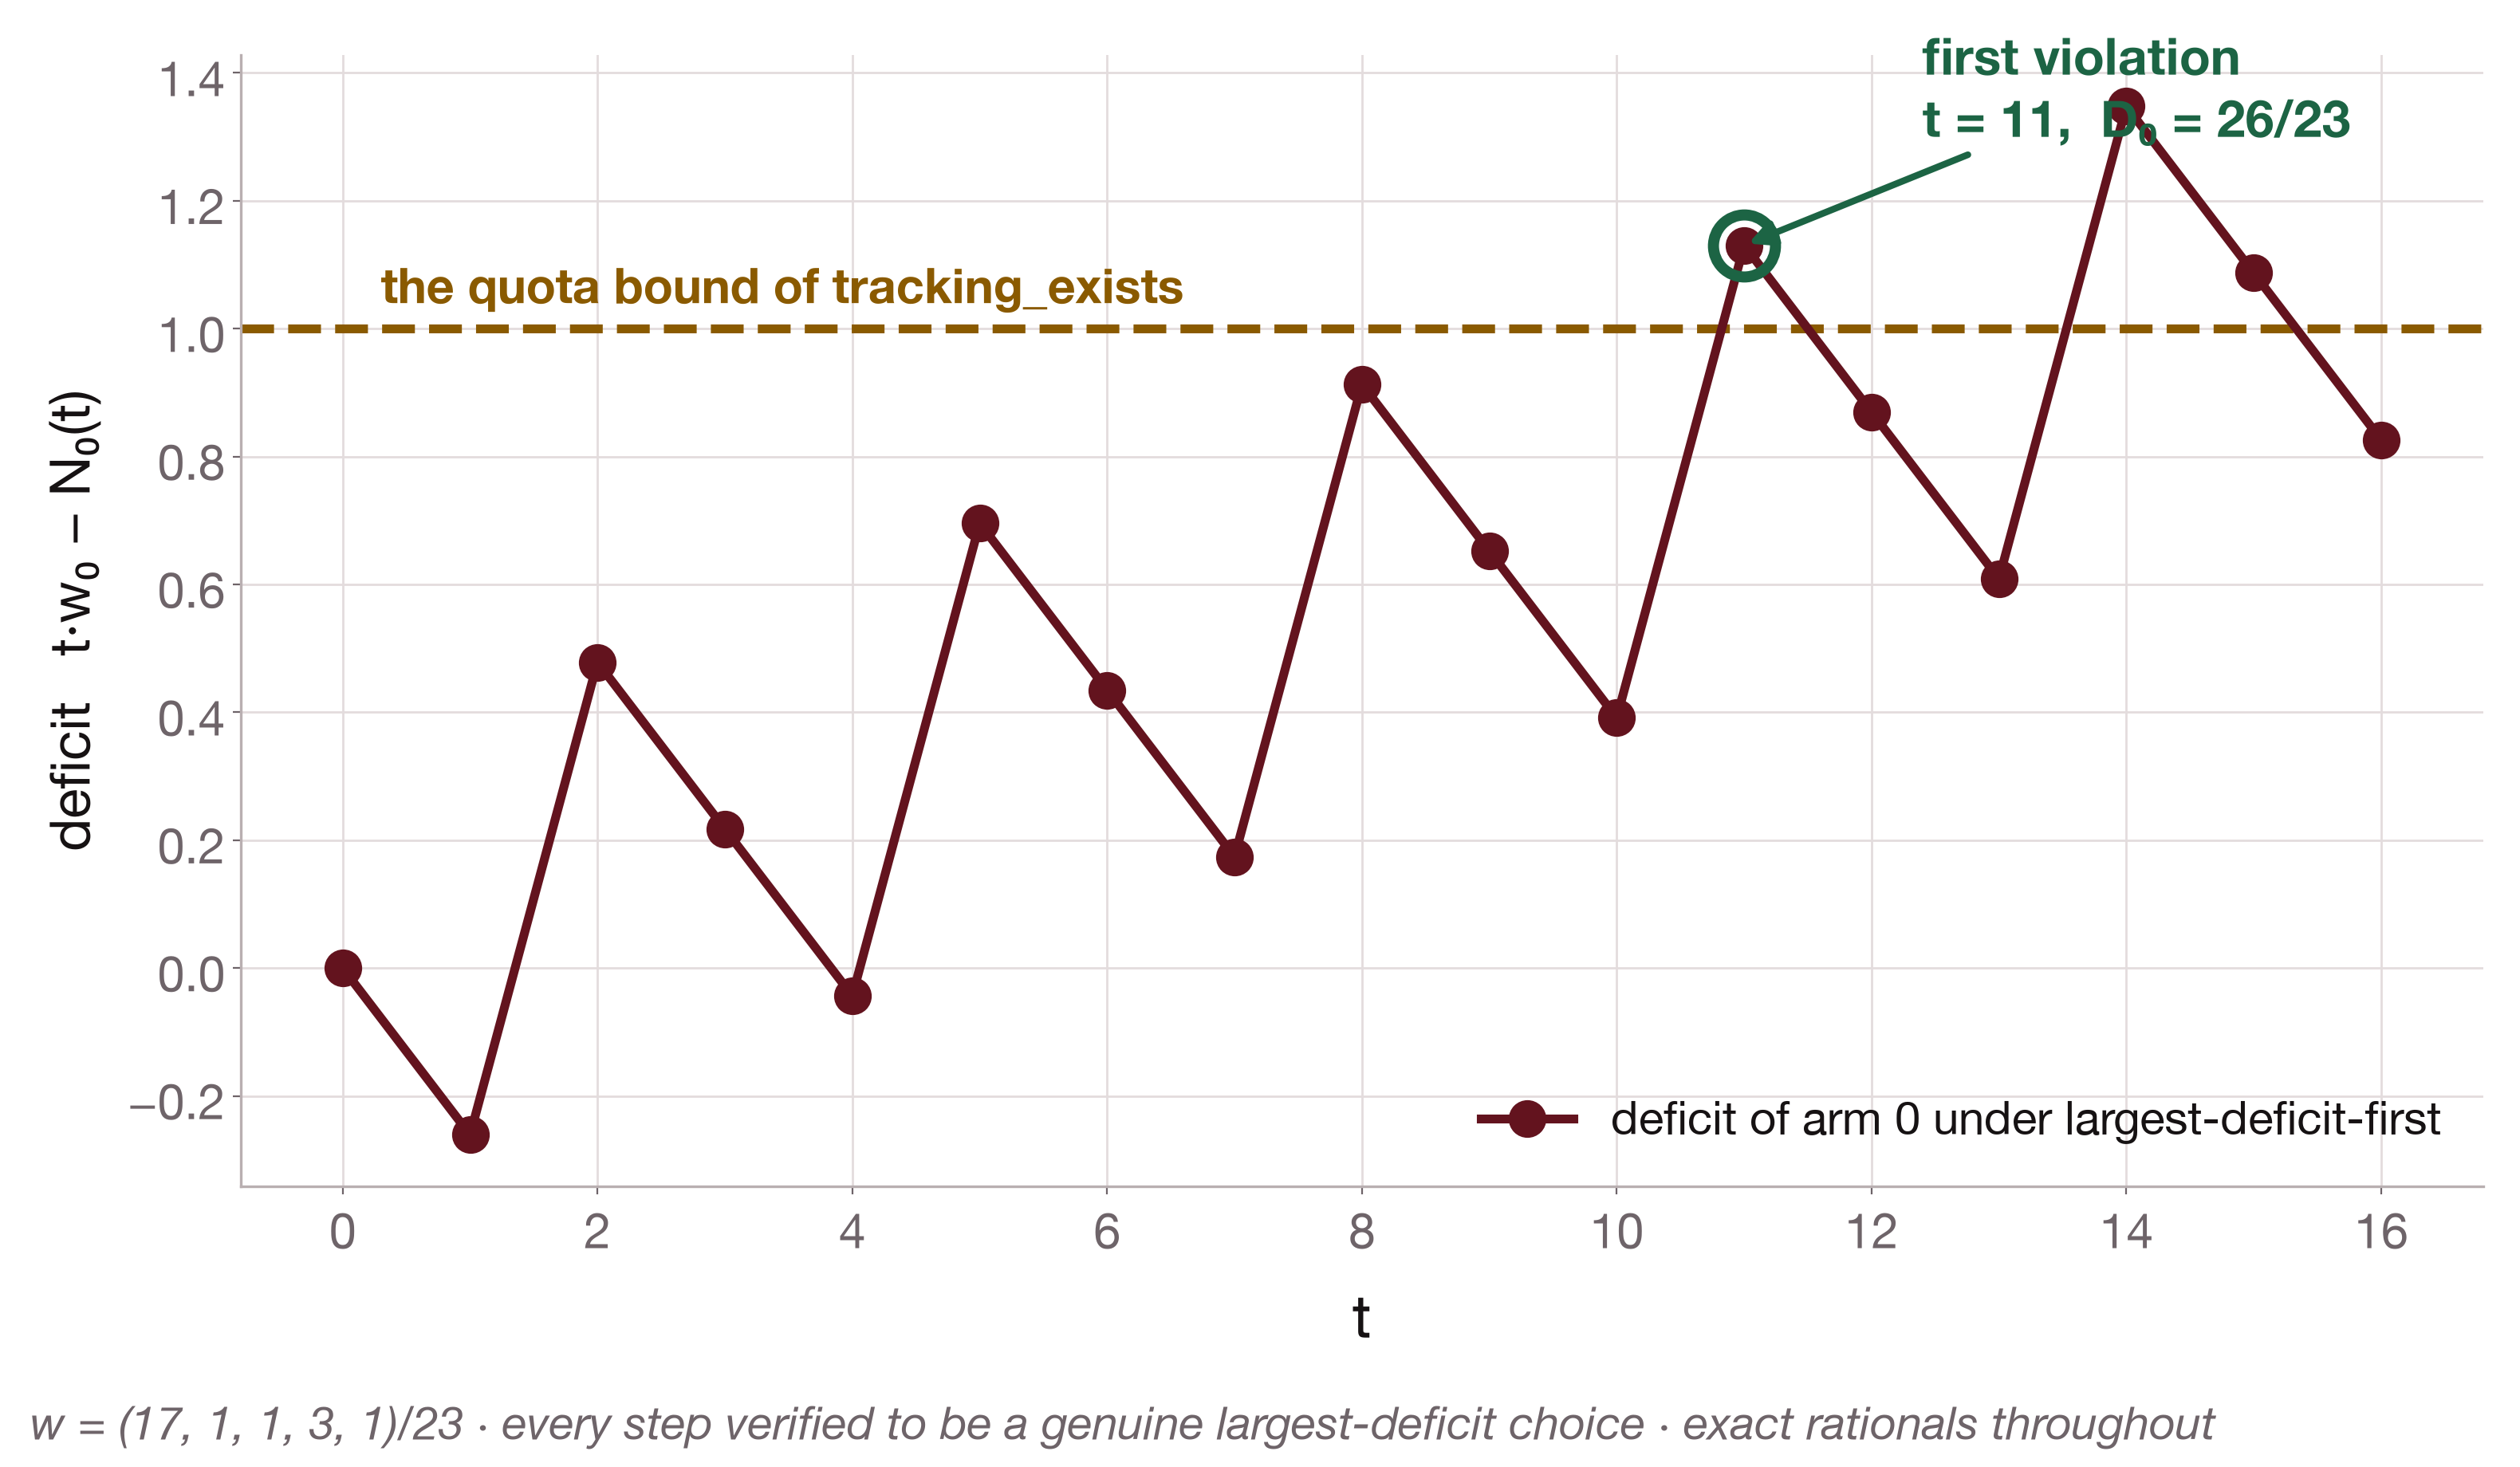
\includegraphics[width=\columnwidth]{adaptive_fig1_quota.png}
\caption{The deficit of the first arm under largest-deficit-first on
$w=\frac{1}{23}(17,1,1,3,1)$. The per-horizon bound of one---achievable offline by
Theorem~\ref{thm:exists}---is crossed at $t=11$ and exceeded thereafter.}
\label{fig:quota}
\end{figure}

\subsection{Skewed Targets Are the Dangerous Ones}

Every one of the ten worst targets has a dominant component above $\tfrac23$ and several
components below $\tfrac{1}{10}$; near-uniform targets do not appear. This matters because
optimal allocations in best-arm identification are typically skewed---budget concentrates on
the arms that are hard to separate---so the regime in which the tracking assumption is least
safe is the regime the algorithm actually operates in. An empirical check on near-uniform
targets would find nothing and would be checking the wrong thing.

\subsection{Reading the Witness}
\label{sec:reading}

The mechanism of the failure is visible in Table~\ref{tab:trace} and is not what one would
guess. The target has one dominant arm and four small ones, so naively the dominant arm should
be served almost every round and its deficit stay small. What happens instead is that each
small arm accumulates deficit slowly until it briefly exceeds the dominant arm's, takes one
sample, and resets---at $t=1,4,7,10$. Each of those is a round the dominant arm does not get,
and its deficit grows by $\tfrac{17}{23}$ meanwhile. After four such interruptions the
shortfall crosses one.

The failure is therefore a property of integrality rather than of greed. The rule always serves
an arm with maximal deficit, which is the locally correct action; the problem is that the unit
of service is one whole sample while the entitlements being balanced are fractions much smaller
than one. Any rule serving whole samples and never revoking them faces the same arithmetic,
which is the content of the apportionment impossibility \cite{balinski1982}. It also explains
the pattern in the search: the worst targets all have several very small components alongside
one dominant one, exactly the configuration in which a small arm's occasional service is most
expensive relative to its entitlement.

\section{Discussion}
\label{sec:discussion}

\subsection{What the Results Establish}

An analysis that assumes an online rule can hold the deficit below one is assuming something
false, and the error is not conservative---it understates how far the realised allocation can
drift, so every bound derived from the intended proportions inherits the understatement in the
wrong direction.

What an analysis may use instead is the per-horizon existence of Theorem~\ref{thm:exists}
together with the transfer of Theorem~\ref{thm:freq}, applied to whatever bound the specific
rule can actually prove. The existence statement is still worth having: it says the target is
not unreachable in principle, so a rule failing to meet it fails for reasons of online-ness
rather than of arithmetic.

Three replacements are available to an implementer, in increasing order of cost. Keep
largest-deficit-first with a larger constant, which must exceed $\tfrac32$ on the searched
family and is not bounded by anything proved here. Use a divisor method, which is
house-monotone with a characterised violation \cite{balinski1982}, at the cost of no longer
serving the largest deficit. Or recompute the allocation from scratch at each horizon using
Theorem~\ref{thm:exists}, which achieves deficit at most one but is not house-monotone---an
arm's count can fall as the horizon grows, which is meaningless once the samples are drawn.
The three exhaust what the obstruction permits.

\subsection{Shortcomings and Limitations}

\emph{One rule, not all rules.} Theorem~\ref{thm:quotafails} refutes the bound $1$ for
\emph{this} rule. It does not prove that no online monotone rule achieves any constant bound,
and the constant for a divisor method is not computed here.

\emph{The rule-to-counts link is not machine-checked.} As Section~\ref{sec:gap} states, the
arithmetic of the violation is proved and the identification of $N$ as the greedy trajectory
rests on an exact recomputation reported here.

\emph{The search covers a finite family.} Rational targets on three to five arms with
denominators to $30$, run to horizon $40$. Nothing here bounds the worst deficit over all
targets, arm counts and horizons, and such a bound---an impossibility with a matching
constant---is the natural companion this paper does not supply.

\emph{A known sub-Gaussian parameter is assumed.} With an estimated variance the hypothesis of
Theorem~\ref{thm:subgauss} is not automatic, and which concentration inequality suffices at the
peeling budget in that case is not settled.

\emph{The geometric tail is an input.} Corollary~\ref{cor:expstop} converts it; establishing it
belongs to the algorithm's own analysis.

\subsection{Open Problems}

Computing the smallest constant achievable online, for a specific rule, would turn
Theorem~\ref{thm:freq} from a template into a bound. Whether $\tfrac32$ is the worst case over
all targets rather than over the searched family is second. Third, the sub-Gaussian hypothesis
with an estimated variance---the setting an implementation actually faces---requires a
different concentration input.

\subsection{Why a Refutation Is Worth Reporting}

Two of this paper's three contributions establish that standard things are true, and the third
establishes that a convenient thing is false. The asymmetry in how they are usually valued is
worth addressing. A refuted assumption is more useful than a confirmed one, because a confirmed
assumption changes no downstream work while a refuted one invalidates results derived from it.
The refutation also comes with a replacement, which is what makes it actionable rather than
merely destructive: the existence theorem says the problem is the online commitment rather than
the arithmetic, and the transfer is stated with the constant free so that an analysis can
substitute what its rule can prove.

The correction is modest in size. An analysis assuming $|D_{i}(t)|\le1$ obtained an
empirical-allocation error of $1/t$; the correct statement carries whatever constant the rule
can prove, which on the searched family exceeds $\tfrac32$. The resulting bound is a constant
factor worse in the term the tracking controls, not asymptotically different. Finding that the
correction is small is a conclusion, not a premise, and it was available only after the
refutation.

\section{Conclusion}

The two probabilistic inputs of the stopping analysis are now theorems: the layer-cake identity
is proved, so a geometric tail bounds the expected stopping time, and the per-arm concentration
inequality is discharged from a sub-Gaussian hypothesis. The tracking question is settled and
the answer is negative: an allocation with deficit at most one exists at every horizon, but the
natural online monotone rule cannot achieve it, and the failure occurs on nearly a quarter of
the targets searched, as early as the third sample, and most severely on exactly the skewed
targets that best-arm identification produces. The broader lesson concerns which parts of an
analysis deserve scrutiny. Of the three inputs closed here, two were true and merely uncited,
so closing them changed nothing except the development's self-sufficiency. The third was false
in the form it was wanted, and no amount of care in the other two would have revealed that.

\section*{Acknowledgment}

The formal development uses the Lean~4 theorem prover and the mathlib library.

\begin{thebibliography}{00}

\bibitem{garivier2016} A. Garivier and E. Kaufmann, ``Optimal best arm identification with
fixed confidence,'' in \emph{Proc. 29th Annu. Conf. Learning Theory (COLT)}, 2016.

\bibitem{kaufmann2016} E. Kaufmann, O. Capp\'e, and A. Garivier, ``On the complexity of
best-arm identification in multi-armed bandit models,'' \emph{J. Mach. Learn. Res.},
vol.~17, pp.~1--42, 2016.

\bibitem{balinski1982} M. L. Balinski and H. P. Young, \emph{Fair Representation: Meeting the
Ideal of One Man, One Vote}. New Haven, CT: Yale Univ. Press, 1982.

\bibitem{boucheron2013} S. Boucheron, G. Lugosi, and P. Massart, \emph{Concentration
Inequalities: A Nonasymptotic Theory of Independence}. Oxford, U.K.: Oxford Univ. Press, 2013.

\bibitem{durrett2019} R. Durrett, \emph{Probability: Theory and Examples}, 5th ed. Cambridge,
U.K.: Cambridge Univ. Press, 2019.

\bibitem{mathlib2020} The mathlib Community, ``The Lean mathematical library,'' in
\emph{Proc. 9th ACM SIGPLAN Int. Conf. Certified Programs and Proofs (CPP)}, 2020,
pp.~367--381.

\bibitem{demoura2021} L. de Moura and S. Ullrich, ``The Lean 4 theorem prover and programming
language,'' in \emph{Proc. 28th Int. Conf. Automated Deduction (CADE)}, 2021, pp.~625--635.

\end{thebibliography}

\appendices
\section{Complete statement inventory}
\label{app:inventory}

This appendix reproduces every axiom-audited theorem and lemma in the Adaptive strand\'s accepted modules---all $26$ of them, grouped by module---so that the corpus behind the paper can be read rather than counted. Each entry is a symbol-level transliteration of the Lean statement: Unicode maps to the corresponding \LaTeX{} symbol and identifiers are set upright, but no structure is rewritten and no hypothesis is dropped. What appears below is what the prover checked.

Binders are listed as the prover has them and the turnstile $\vdash$ separates them from the conclusion. Every entry carries an acceptance receipt and an axiom audit confining it to $\{\textsf{propext},\textsf{Classical.choice},\textsf{Quot.sound}\}$; none contains \texttt{sorry}.

\vspace{4pt}\noindent\rule{\columnwidth}{0.4pt}\par\vspace{2pt}
\noindent\textbf{Module \lean{LeanAdaptiveConfidenceJoinV1}}\par\vspace{3pt}

\noindent\textbf{A\,1}\quad\lean{cost\_on\_event}
{\footnotesize\[ \begin{aligned}[t]
&\{ \mathit{E} : \mathit{Prop}\},\; (\mathit{b0} \mathit{Bstar} : \mathbb{R} ),\; (\mathit{hb0} : 0 <\\
&\quad \mathit{b0}),\; (\mathit{hB} : \mathit{b0} \leq \mathit{Bstar}),\; (\mathit{k} : \mathbb{N}\\
&\quad ),\; (\mathit{hk} : \mathit{Bstar} \leq \mathit{budget} \mathit{b0} \mathit{k}),\; (\mathit{hmin} : \forall \mathit{j}, \mathit{j} < \mathit{k} \to \mathit{budget} \mathit{b0} \mathit{j} <\\
&\quad \mathit{Bstar}),\; (\mathit{hE} : \mathit{E})
\end{aligned} \]}
{\footnotesize\[ \begin{aligned}[t]
\vdash\;&\textstyle\sum \mathit{i} \in \mathit{Finset}.\mathit{range} (\mathit{k} + 1),\\
&\quad \mathit{budget} \mathit{b0} \mathit{i} < 4 * \mathit{Bstar}
\end{aligned} \]}

\vspace{4pt}\noindent\rule{\columnwidth}{0.4pt}\par\vspace{2pt}
\noindent\textbf{Module \lean{LeanAdaptiveExpectedStoppingV1}}\par\vspace{3pt}

\noindent\textbf{A\,2}\quad\lean{expected\_stopping\_le}
{\footnotesize\[ \begin{aligned}[t]
&(\mu : \mathit{Measure} \Omega ),\; (\mathit{tau} : \Omega \to \mathbb{N} ),\; (\mathit{hmeas} : \mathit{Measurable}\\
&\quad \mathit{tau}),\; (\mathit{C} \mathit{rho} : \mathbb{R}_{\geq0}^{\infty} ),\; (\mathit{hrho} : \mathit{rho} <\\
&\quad 1),\; (\mathit{htail} : \forall \mathit{n} : \mathbb{N} , \mu \{ \omega | \mathit{n} < \mathit{tau} \omega \} \leq \mathit{C} * \mathit{rho}\\
&\quad ^{\mathit{n}})
\end{aligned} \]}
{\footnotesize\[ \begin{aligned}[t]
\vdash\;&\int^{-} \omega , (\mathit{tau} \omega : \mathbb{R}_{\geq0}^{\infty} ) ∂\mu \leq \mathit{C}\\
&\quad * (1 - \mathit{rho})^{-1}
\end{aligned} \]}

\noindent\textbf{A\,3}\quad\lean{lintegral\_nat\_eq\_tsum\_meas\_gt}
{\footnotesize\[ \begin{aligned}[t]
&(\mu : \mathit{Measure} \Omega ),\; (\mathit{tau} : \Omega \to \mathbb{N} ),\; (\mathit{hmeas} : \mathit{Measurable}\\
&\quad \mathit{tau})
\end{aligned} \]}
{\footnotesize\[ \begin{aligned}[t]
\vdash\;&\int^{-} \omega , (\mathit{tau} \omega : \mathbb{R}_{\geq0}^{\infty} ) ∂\mu = \textstyle\sum '\\
&\quad \mathit{n} : \mathbb{N} , \mu \{ \omega | \mathit{n} < \mathit{tau} \omega \}
\end{aligned} \]}

\noindent\textbf{A\,4}\quad\lean{subgaussian\_threshold}
{\footnotesize\[ \begin{aligned}[t]
&\{ \mu : \mathit{Measure} \Omega \},\; [\mathit{IsProbabilityMeasure} \mu ],\; \{ \mathit{X}\\
&\quad : \Omega \to \mathbb{R} \},\; \{ \mathit{c} : \mathbb{R}_{\geq0} \},\; (\mathit{hc} : (0:\mathbb{R} ) < (\mathit{c} : \mathbb{R}\\
&\quad )),\; (\mathit{h} : \mathit{HasSubgaussianMGF} \mathit{X} \mathit{c} \mu ),\; (\mathit{beta} : \mathbb{R}\\
&\quad ),\; (\mathit{hb0} : 0 < \mathit{beta}),\; (\mathit{hb1} : \mathit{beta} \leq 1)
\end{aligned} \]}
{\footnotesize\[ \begin{aligned}[t]
\vdash\;&\mu .\mathit{real} \{ \omega | \mathit{Real}.\mathit{sqrt} (2 * (\mathit{c} : \mathbb{R} ) * \mathit{Real}.\mathit{log} (1 /\\
&\quad \mathit{beta})) \leq \mathit{X} \omega \} \leq \mathit{beta}
\end{aligned} \]}

\vspace{4pt}\noindent\rule{\columnwidth}{0.4pt}\par\vspace{2pt}
\noindent\textbf{Module \lean{LeanAdaptiveLoopJoinV1}}\par\vspace{3pt}

\noindent\textbf{A\,5}\quad\lean{doubling\_factor}
{\footnotesize\[ \begin{aligned}[t]
&(\mathit{b0} \mathit{Bstar} : \mathbb{R} ),\; (\mathit{hb0} : 0 < \mathit{b0}),\; (\mathit{hB} : \mathit{b0} \leq \mathit{Bstar}),\; (\mathit{k} : \mathbb{N}\\
&\quad ),\; (\mathit{hk} : \mathit{Bstar} \leq \mathit{budget} \mathit{b0} \mathit{k}),\; (\mathit{hmin} : \forall \mathit{j}, \mathit{j} < \mathit{k} \to \mathit{budget} \mathit{b0} \mathit{j} <\\
&\quad \mathit{Bstar})
\end{aligned} \]}
{\footnotesize\[ \begin{aligned}[t]
\vdash\;&\textstyle\sum \mathit{i} \in \mathit{Finset}.\mathit{range} (\mathit{k} + 1),\\
&\quad \mathit{budget} \mathit{b0} \mathit{i} < 4 * \mathit{Bstar}
\end{aligned} \]}

\noindent\textbf{A\,6}\quad\lean{late\_revalidation\_can\_overshoot}
{\footnotesize\[ \begin{aligned}[t]
&(\mathit{b0} : \mathbb{R} ),\; (\mathit{hb0} : 0 < \mathit{b0}),\; (\mathit{m} : \mathbb{N}\\
&\quad )
\end{aligned} \]}
{\footnotesize\[ \begin{aligned}[t]
\vdash\;&\mathit{budget} \mathit{b0} \mathit{m} = 2 ^{\mathit{m}} * \mathit{budget} \mathit{b0} 0
\end{aligned} \]}

\noindent\textbf{A\,7}\quad\lean{total\_le\_two\_last}
{\footnotesize\[ \begin{aligned}[t]
&(\mathit{b0} : \mathbb{R} ),\; (\mathit{hb} : 0 \leq \mathit{b0}),\; (\mathit{K} : \mathbb{N}\\
&\quad )
\end{aligned} \]}
{\footnotesize\[ \begin{aligned}[t]
\vdash\;&\textstyle\sum \mathit{k} \in \mathit{Finset}.\mathit{range} (\mathit{K} + 1),\\
&\quad \mathit{budget} \mathit{b0} \mathit{k} \leq 2 * \mathit{budget} \mathit{b0} \mathit{K}
\end{aligned} \]}

\noindent\textbf{A\,8}\quad\lean{two\_pow\_sum}
{\footnotesize\[ \begin{aligned}[t]
&(\mathit{K} : \mathbb{N} )
\end{aligned} \]}
{\footnotesize\[ \begin{aligned}[t]
\vdash\;&\textstyle\sum \mathit{k} \in \mathit{Finset}.\mathit{range} (\mathit{K} + 1), (2:\mathbb{R}\\
&\quad ) ^{\mathit{k}} = 2 ^{} (\mathit{K} + 1) - 1
\end{aligned} \]}

\vspace{4pt}\noindent\rule{\columnwidth}{0.4pt}\par\vspace{2pt}
\noindent\textbf{Module \lean{LeanAdaptiveOnlineQuotaFailsV1}}\par\vspace{3pt}

\noindent\textbf{A\,9}\quad\lean{counts\_sum}
{\footnotesize\[ \begin{aligned}[t]
\vdash\;&\textstyle\sum \mathit{i}, \mathit{N} \mathit{i} = 11
\end{aligned} \]}

\noindent\textbf{A\,10}\quad\lean{deficit\_exceeds\_one}
{\footnotesize\[ \begin{aligned}[t]
\vdash\;&(1 : \mathbb{Q} ) < (11 : \mathbb{Q} ) * \mathit{w} 0 - (\mathit{N} 0 : \mathbb{Q} )
\end{aligned} \]}

\noindent\textbf{A\,11}\quad\lean{greedy\_steps}
{\footnotesize\[ \begin{aligned}[t]
\vdash\;&\mathit{True}
\end{aligned} \]}

\noindent\textbf{A\,12}\quad\lean{online\_quota\_fails}
{\footnotesize\[ \begin{aligned}[t]
\vdash\;&(\textstyle\sum \mathit{i}, \mathit{w} \mathit{i} = 1)\\
&\quad \wedge (\textstyle\sum \mathit{i}, \mathit{N} \mathit{i} = 11)\\
&\quad \wedge (1 : \mathbb{Q} ) < (11 : \mathbb{Q} ) * \mathit{w} 0 - (\mathit{N} 0 : \mathbb{Q} )
\end{aligned} \]}

\noindent\textbf{A\,13}\quad\lean{weights\_sum\_one}
{\footnotesize\[ \begin{aligned}[t]
\vdash\;&\textstyle\sum \mathit{i}, \mathit{w} \mathit{i} = 1
\end{aligned} \]}

\vspace{4pt}\noindent\rule{\columnwidth}{0.4pt}\par\vspace{2pt}
\noindent\textbf{Module \lean{LeanAdaptiveStoppingTailV1}}\par\vspace{3pt}

\noindent\textbf{A\,14}\quad\lean{expectation\_of\_tail}
{\footnotesize\[ \begin{aligned}[t]
&(\mathit{C} \mathit{rho} : \mathbb{R} ),\; (\mathit{tail} : \mathbb{N} \to \mathbb{R} ),\; (\mathit{hC} : 0 \leq \mathit{C}),\; (\mathit{h0} : 0 \leq \mathit{rho}),\; (\mathit{h1} : \mathit{rho} <\\
&\quad 1),\; (\mathit{hnn} : \forall \mathit{n}, 0 \leq \mathit{tail} \mathit{n}),\; (\mathit{hle} : \forall \mathit{n}, \mathit{tail} \mathit{n} \leq \mathit{C} * \mathit{rho}\\
&\quad ^{\mathit{n}}),\; (\mathit{hsum} : \mathit{Summable} \mathit{tail})
\end{aligned} \]}
{\footnotesize\[ \begin{aligned}[t]
\vdash\;&\textstyle\sum ' \mathit{n} : \mathbb{N} , \mathit{tail} \mathit{n}\\
&\quad \leq \mathit{C} / (1 - \mathit{rho})
\end{aligned} \]}

\noindent\textbf{A\,15}\quad\lean{geometric\_tail\_sum}
{\footnotesize\[ \begin{aligned}[t]
&(\mathit{C} \mathit{rho} : \mathbb{R} ),\; (\mathit{hC} : 0 \leq \mathit{C}),\; (\mathit{h0} : 0 \leq \mathit{rho}),\; (\mathit{h1} : \mathit{rho} <\\
&\quad 1)
\end{aligned} \]}
{\footnotesize\[ \begin{aligned}[t]
\vdash\;&\textstyle\sum ' \mathit{n} : \mathbb{N} , \mathit{C} * \mathit{rho} ^{\mathit{n}}\\
&\quad = \mathit{C} / (1 - \mathit{rho})
\end{aligned} \]}

\noindent\textbf{A\,16}\quad\lean{grid\_overhead}
{\footnotesize\[ \begin{aligned}[t]
&(\mathit{eps} \mathit{b0} \mathit{Bstar} \mathit{target} \mathit{prev} : \mathbb{R} ),\; (\mathit{heps} : 0 <\\
&\quad \mathit{eps}),\; (\mathit{hb0} : 0 < \mathit{b0}),\; (\mathit{hB} : 0 < \mathit{Bstar}),\; (\mathit{hprev} : \mathit{prev} <\\
&\quad \mathit{Bstar}),\; (\mathit{hstep} : \mathit{target} \leq (1 + \mathit{eps}) * \mathit{prev} +\\
&\quad \mathit{b0})
\end{aligned} \]}
{\footnotesize\[ \begin{aligned}[t]
\vdash\;&\mathit{target} < (1 + \mathit{eps}) * \mathit{Bstar} + \mathit{b0}
\end{aligned} \]}

\noindent\textbf{A\,17}\quad\lean{peeling\_budget}
{\footnotesize\[ \begin{aligned}[t]
&(\mathit{K} : \mathbb{N} ),\; (\mathit{hK} : 0 < \mathit{K}),\; (\mathit{delta} : \mathbb{R}\\
&\quad ),\; (\mathit{N} : \mathbb{N} )
\end{aligned} \]}
{\footnotesize\[ \begin{aligned}[t]
\vdash\;&\textstyle\sum \mathit{n} \in \mathit{Finset}.\mathit{range} \mathit{N}, (\mathit{K} : \mathbb{R}\\
&\quad ) * (\mathit{delta} / ((\mathit{K} : \mathbb{R} ) * ((\mathit{n} + 1) * (\mathit{n} + 2))))\\
&\quad = \mathit{delta} * (1 - 1 / ((\mathit{N} : \mathbb{R} ) + 1))
\end{aligned} \]}

\noindent\textbf{A\,18}\quad\lean{telescope\_limit}
{\footnotesize\[ \begin{aligned}[t]
\vdash\;&\mathit{Filter}.\mathit{Tendsto} (\mathbf{fun} \mathit{N} : \mathbb{N} => \textstyle\sum \mathit{n} \in \mathit{Finset}.\mathit{range} \mathit{N}, (1 : \mathbb{R} ) / ((\mathit{n} + 1) * (\mathit{n} +\\
&\quad 2))) \mathit{Filter}.\mathit{atTop} (\mathit{nhds} 1)
\end{aligned} \]}

\noindent\textbf{A\,19}\quad\lean{telescope\_partial}
{\footnotesize\[ \begin{aligned}[t]
&(\mathit{N} : \mathbb{N} )
\end{aligned} \]}
{\footnotesize\[ \begin{aligned}[t]
\vdash\;&\textstyle\sum \mathit{n} \in \mathit{Finset}.\mathit{range} \mathit{N}, (1 : \mathbb{R} ) / ((\mathit{n} + 1) * (\mathit{n} +\\
&\quad 2)) = 1 - 1 / (\mathit{N} + 1)
\end{aligned} \]}

\noindent\textbf{A\,20}\quad\lean{union\_bound}
{\footnotesize\[ \begin{aligned}[t]
&\{ \Omega : \mathit{Type}*\},\; [\mathit{MeasurableSpace} \Omega ],\; (\mu : \mathit{Measure} \Omega ),\; (\mathit{B} : \mathbb{N} \to \mathit{Set} \Omega ),\; (\mathit{d} : \mathbb{N} \to \mathbb{R}_{\geq0}^{\infty}\\
&\quad ),\; (\mathit{delta} : \mathbb{R}_{\geq0}^{\infty} ),\; (\mathit{hB} : \forall \mathit{n}, \mu (\mathit{B} \mathit{n}) \leq \mathit{d}\\
&\quad \mathit{n}),\; (\mathit{hd} : \textstyle\sum ' \mathit{n}, \mathit{d} \mathit{n} \leq \mathit{delta})
\end{aligned} \]}
{\footnotesize\[ \begin{aligned}[t]
\vdash\;&\mu (⋃ \mathit{n}, \mathit{B} \mathit{n}) \leq \mathit{delta}
\end{aligned} \]}

\vspace{4pt}\noindent\rule{\columnwidth}{0.4pt}\par\vspace{2pt}
\noindent\textbf{Module \lean{LeanAdaptiveTrackingV1}}\par\vspace{3pt}

\noindent\textbf{A\,21}\quad\lean{deficit\_sum\_zero}
{\footnotesize\[ \begin{aligned}[t]
&(\mathit{w} : \iota \to \mathbb{R} ),\; (\mathit{N} : \iota \to \mathbb{N} ),\; (\mathit{t} : \mathbb{N}\\
&\quad ),\; (\mathit{hw} : \textstyle\sum \mathit{i}, \mathit{w} \mathit{i} = 1),\; (\mathit{hN} : \textstyle\sum \mathit{i}, \mathit{N} \mathit{i} =\\
&\quad \mathit{t})
\end{aligned} \]}
{\footnotesize\[ \begin{aligned}[t]
\vdash\;&\textstyle\sum \mathit{i}, \mathit{deficit} \mathit{w} \mathit{N} \mathit{t} \mathit{i}\\
&\quad = 0
\end{aligned} \]}

\noindent\textbf{A\,22}\quad\lean{exists\_deficient}
{\footnotesize\[ \begin{aligned}[t]
&[\mathit{Nonempty} \iota ],\; (\mathit{w} : \iota \to \mathbb{R} ),\; (\mathit{N} : \iota \to \mathbb{N}\\
&\quad ),\; (\mathit{t} : \mathbb{N} ),\; (\mathit{hw} : \textstyle\sum \mathit{i}, \mathit{w} \mathit{i} =\\
&\quad 1),\; (\mathit{hN} : \textstyle\sum \mathit{i}, \mathit{N} \mathit{i} = \mathit{t})
\end{aligned} \]}
{\footnotesize\[ \begin{aligned}[t]
\vdash\;&\exists \mathit{i}, 0 \leq \mathit{deficit} \mathit{w} \mathit{N} \mathit{t} \mathit{i}
\end{aligned} \]}

\noindent\textbf{A\,23}\quad\lean{frequency\_converges}
{\footnotesize\[ \begin{aligned}[t]
&(\mathit{w} : \iota \to \mathbb{R} ),\; (\mathit{N} : \iota \to \mathbb{N} ),\; (\mathit{t} : \mathbb{N}\\
&\quad ),\; (\mathit{c} : \mathbb{R} ),\; (\mathit{ht} : 0 < \mathit{t}),\; (\mathit{hc} : \forall \mathit{i}, |(\mathit{N} \mathit{i} : \mathbb{R} ) - (\mathit{t} : \mathbb{R} ) * \mathit{w} \mathit{i}| \leq \mathit{c}),\; (\mathit{i} : \iota )
\end{aligned} \]}
{\footnotesize\[ \begin{aligned}[t]
\vdash\;&|(\mathit{N} \mathit{i} : \mathbb{R} ) / (\mathit{t} : \mathbb{R} ) - \mathit{w} \mathit{i}|\\
&\quad \leq \mathit{c} / (\mathit{t} : \mathbb{R} )
\end{aligned} \]}

\noindent\textbf{A\,24}\quad\lean{pull\_count\_lower}
{\footnotesize\[ \begin{aligned}[t]
&(\mathit{w} : \iota \to \mathbb{R} ),\; (\mathit{s} \mathit{t} : \mathbb{N} ),\; (\mathit{c} : \mathbb{R}\\
&\quad ),\; (\mathit{i} : \iota ),\; (\mathit{Ns} \mathit{Nt} : \mathbb{R} ),\; (\mathit{hNs} : |\mathit{Ns} - (\mathit{s} : \mathbb{R} ) * \mathit{w} \mathit{i}| \leq \mathit{c}),\; (\mathit{hNt} : |\mathit{Nt} - (\mathit{t} : \mathbb{R} ) * \mathit{w} \mathit{i}| \leq \mathit{c})
\end{aligned} \]}
{\footnotesize\[ \begin{aligned}[t]
\vdash\;&((\mathit{t} : \mathbb{R} ) - (\mathit{s} : \mathbb{R} )) * \mathit{w} \mathit{i} - 2 *\\
&\quad \mathit{c} \leq \mathit{Nt} - \mathit{Ns}
\end{aligned} \]}

\noindent\textbf{A\,25}\quad\lean{tracking\_bound}
{\footnotesize\[ \begin{aligned}[t]
&(\mathit{w} : \iota \to \mathbb{R} ),\; (\mathit{N} : \iota \to \mathbb{N} ),\; (\mathit{t} : \mathbb{N}\\
&\quad ),\; (\mathit{hlo} : \forall \mathit{i}, ((\lfloor (\mathit{t} : \mathbb{R} ) * \mathit{w} \mathit{i}\rfloor : \mathbb{Z} ) : \mathbb{R} ) \leq (\mathit{N} \mathit{i} : \mathbb{R}\\
&\quad )),\; (\mathit{hhi} : \forall \mathit{i}, (\mathit{N} \mathit{i} : \mathbb{R} ) \leq ((\lfloor (\mathit{t} : \mathbb{R} ) * \mathit{w} \mathit{i}\rfloor : \mathbb{Z} ) : \mathbb{R} ) +\\
&\quad 1),\; (\mathit{i} : \iota )
\end{aligned} \]}
{\footnotesize\[ \begin{aligned}[t]
\vdash\;&|(\mathit{N} \mathit{i} : \mathbb{R} ) - (\mathit{t} : \mathbb{R} ) * \mathit{w} \mathit{i}|\\
&\quad \leq 1
\end{aligned} \]}

\noindent\textbf{A\,26}\quad\lean{tracking\_exists}
{\footnotesize\[ \begin{aligned}[t]
&[\mathit{Nonempty} \iota ],\; (\mathit{w} : \iota \to \mathbb{R} ),\; (\mathit{t} : \mathbb{N}\\
&\quad ),\; (\mathit{hw} : \textstyle\sum \mathit{i}, \mathit{w} \mathit{i} = 1),\; (\mathit{hw0} : \forall \mathit{i}, 0 \leq \mathit{w}\\
&\quad \mathit{i})
\end{aligned} \]}
{\footnotesize\[ \begin{aligned}[t]
\vdash\;&\exists \mathit{N} : \iota \to \mathbb{N} , (\textstyle\sum \mathit{i}, \mathit{N} \mathit{i} =\\
&\quad \mathit{t}) \wedge \forall \mathit{i}, |(\mathit{N} \mathit{i} : \mathbb{R} ) - (\mathit{t} : \mathbb{R}\\
&\quad ) * \mathit{w} \mathit{i}| \leq 1
\end{aligned} \]}


\end{document}
